\documentclass[a4paper, 11pt]{article}
\usepackage[utf8]{inputenc}
\usepackage[english]{babel}
\usepackage{pgfplots}
\pgfplotsset{width=10cm,compat=1.9}

%Margins 
\usepackage[a4paper, left=1.27cm,top=1.27cm,right =1.27cm, bottom = 1.4cm]{geometry}

%Load packages
%Algemene packages
\usepackage{babel}
\usepackage{slantsc}
\usepackage{array}
\renewcommand{\arraystretch}{2}
\usepackage{multicol}
\usepackage{multirow}
\usepackage{amsmath}
\usepackage{amsfonts}
\usepackage{booktabs}

%Opsommingen
\usepackage{enumerate}


%Afbeeldingen
\usepackage{graphicx}
\usepackage{wrapfig}

%Gekleurde tekstboxen 
\usepackage[most]{tcolorbox}

%Stop indent
\setlength{\parindent}{0pt}

%Font
\usepackage{cmbright}
\usepackage[OT1]{fontenc}

%Headers and footers
\usepackage{fancyhdr}

\pagestyle{fancy}
\fancyhf{}
\renewcommand{\headrulewidth}{0pt}
\renewcommand{\footrulewidth}{0pt}
\fancyhead[LE,RO]{}
\fancyhead[RE,LO]{}

%Logo in footer
\usepackage{lastpage}
\lfoot{}
\cfoot{\vspace{-5mm} \thepage}
\rfoot{}

%Voorbeeldtekst
\usepackage{lipsum}

%Meerdere kolommen
\usepackage{multicol}
\setlength{\columnsep}{1cm}

%Whitespace na section
\usepackage[compact]{titlesec}  
\titlespacing{\section}{0pt}{2pt}{0pt}

%Tekst kleur
\usepackage{xcolor}

%Nieuwe kleur
%\definecolor{ugent_blue}{rgb}{0.04706, 0.13725, 0.26667}
\definecolor{ugent_blue}{RGB}{30, 100, 200}

%Nummering sections
\renewcommand\thesection{\arabic{section}}
\renewcommand\thesubsection{\thesection.\arabic{subsection}}

%Lay-out hoofdingen
\titleformat*{\section}{\bfseries \normalfont}
\usepackage{sectsty}
\sectionfont{\color{ugent_blue}}
\titlespacing\section{0pt}{10pt plus 4pt minus 4pt}{0pt plus 2pt minus 2pt}

\raggedbottom


%other shit that may be useful
\usepackage{multicol,caption}
\usepackage{mathtools}
\raggedbottom
\newcommand{\HRule}{\hrule}
\abovedisplayskip0pt
\renewcommand{\arraystretch}{1.5}
\newcolumntype{M}[1]{>{\centering\arraybackslash}m{#1}}
\usepackage{lscape}
\newenvironment{Figure}
  {\par\medskip\noindent\minipage{\linewidth}}
  {\endminipage\par\medskip}
\usepackage{float}
\usepackage{hyperref}
\newcommand\myfigure[1]{%
\medskip\noindent\begin{minipage}{\columnwidth}
\centering%
#1%
%figure,caption, and label go here
\end{minipage}\medskip}
\usepackage{caption}
\usepackage{subcaption}
\usepackage{tabularx}
\usepackage{enumerate}
\usepackage{enumitem}

\raggedbottom
\raggedcolumns


\graphicspath{{figures/}}

%units
\newcommand{\MW}{\frac{\text{g}}{\text{mol}}}
\newcommand{\g}{\text{g}}
\newcommand{\ml}{\text{ml}}
\newcommand{\density}{\frac{\text{g}}{\text{ml}}}
\newcommand{\mole}{\text{mol}}
%symbols
\newcommand{\mathtext}[2][]{\text{#2}_{\text{#1}}}

%citing
\newcommand{\citec}[1]{{\color{ugent_blue}\cite{#1}}}

%glossary
\usepackage[stylemods=longbooktabs,automake]{glossaries-extra}
\usepackage{glossary-inline}

\makeglossaries

\newabbreviation{pla}{PLA}{polylactic acid}
\newabbreviation{plla}{PLLA}{poly L-lactic acid}
\newabbreviation{la}{LA}{lactic acid}
\newabbreviation{rop}{ROP}{ring opening polymerisation}
\newabbreviation{pdla}{PDLA}{poly D-lactic acid}
\newabbreviation{pdlla}{PDLLA}{poly DL-lactic acid}
\newabbreviation{ap}{AP}{azeotropic polycondensation}
\newabbreviation{ssp}{SSP}{solid state polycondensation}
\newabbreviation{tga}{TGA}{thermogravimetric analysis}
\newabbreviation{dsc}{DSC}{differential scanning calorimetry}

\glssetcategoryattribute{acronym}{indexonlyfirst}{true}
\renewcommand*{\glsinlinenameformat}[2]{\glstarget{#1}{\textsc{#2}}}
\setglossarystyle{inline}

\begin{document}

%Load heading of document
%ugent color
{\color{ugent_blue} \hrule\hrule\hrule}

\vspace*{-0.43mm}
\colorbox{ugent_blue}{\color{white} \bf Report Biomechanics}\\

\noindent\begin{minipage}{0.7\textwidth}% adapt widths of minipages to your needs
{\LARGE \bf \color{ugent_blue} Clinical Movement Analysis Lab Assignment 2022}\\[2mm]

%
{\large Vincent Belpaire}\\
{Supervisor: Prof. Malcolm Forward}\\


{\small University of Ghent}\\
{\small Faculty of Engineering and Architecture}\\
{\small Bachelor of Science: Biomedical Engineering}\\
\end{minipage}%
\hfill%
\begin{minipage}{0.3\textwidth}
\vspace{-2.2cm}
\begin{center}

\includegraphics[width=\linewidth]{ugent_logo}
\end{center}
\end{minipage}\\

\printglossaries

\section{Reaction mechanism of the fabrication methods for PLA}

A very common used bio-based polymer is \gls{pla}. The two best know pathways to synthesize \gls{pla} are via a \gls{rop} or polycondensation. 
These two different routes to form \gls{pla} start from the monomer \gls{la} for which two optically active stereoisomers exists, namely the naturally occuring L-\gls{la} (S configuration) and the manufactured D-\gls{la} (R-configuration)(fig. \ref{fig:LA_types}). 
Pure L- and D-\gls{la} are generally synthesized by fermentation using suitable micro-organisms but the recamic DL-\gls{la} (RS configuration) is conventiently synthesize by a chemical method and shows some characteristic differences from the optically active ones\citec{MASUTANI201411}.

\begin{figure}[ht]
    \centering
    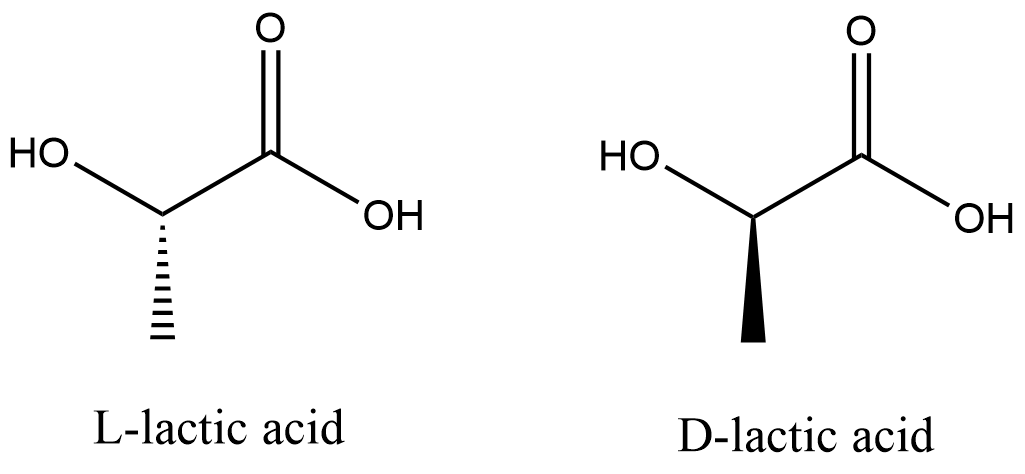
\includegraphics[width=0.5\textwidth]{LA_types.png}
    \caption{L-LA (left) and D-LA (right)}
    \label{fig:LA_types}
\end{figure}

\subsection{Ring opening polymerisation}

Industrial production of \gls{pla} mostly depends on \gls{rop}. This polymerisation reaction starts from lactide which is created starting from \gls{la}. 
There exists three lactides consisting of different stereoisomeric \gls{la} units, namely L-, D- and meso-lactide.  
L- and D-lactides consist of two L- and D-\gls{la}s, respectively, while meso-lactide consists of both L- and D-\gls{la}. Racemic lactide (rac-lactide) is an equimolar mixture of L- and D-lactides\citec{MASUTANI201411}.

\begin{figure}[ht]
    \centering
    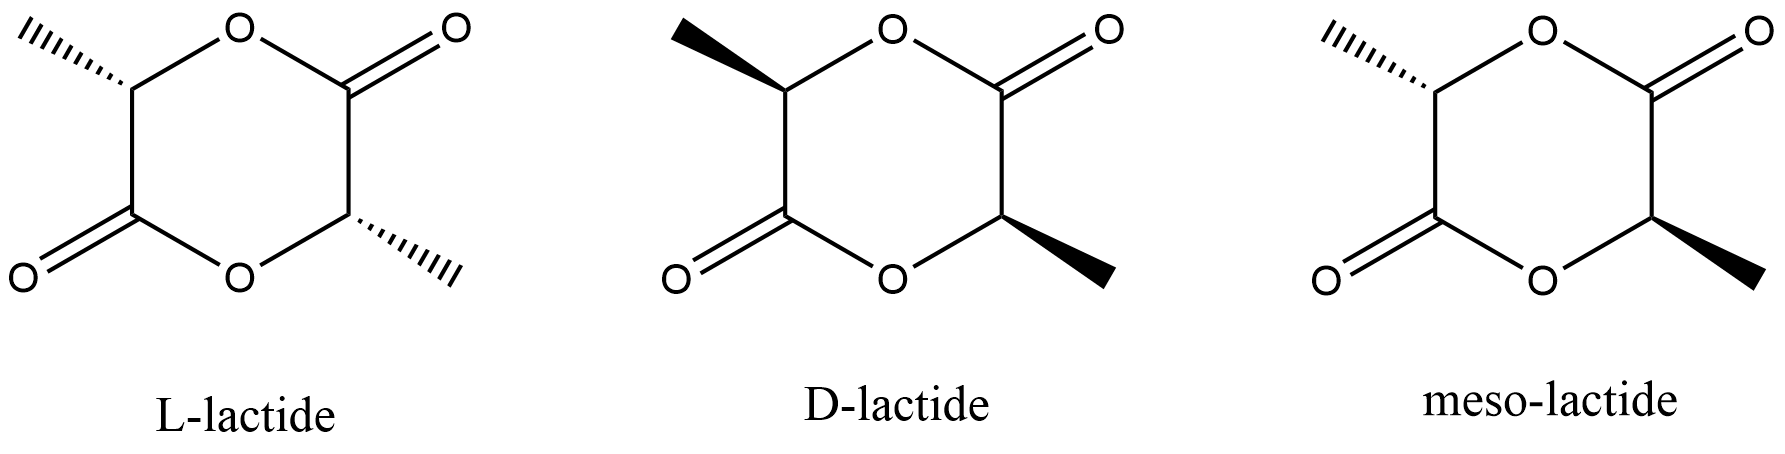
\includegraphics[width=0.8\textwidth]{lactide_types.png}
    \caption{L-lactide (left), D-lactide (middle) and meso-lactide (right)}
    \label{fig:lactide_types}
\end{figure}

The polymerisation of L- and D-lactides gives isotactic homopolymers of \gls{plla} and \gls{pdla}, respectively. Using rac- and meso-lactides for the polymerisation results in optically inactive \gls{pdlla} which has an atactic sequence of L and D units\citec{MASUTANI201411}.

Three reaction mechanisms have been proposed thus far for ROP of lactide: namely anionic, cationic and coordination (also called radical) mechanisms. The anionic and cationic mechanisms have some undesirable side effects and for that reason the coordination mechanism is mostly used. 
Coordination polymerisation with a metal catalyst (mostly alkoxides) can give large molecular weight with a high optical purity. The main principle of how this reaction occurs is seen in figure \ref{fig:PLA_ROP}. (n denotes the amout of lactides added)

\begin{figure}[ht]
    \centering
    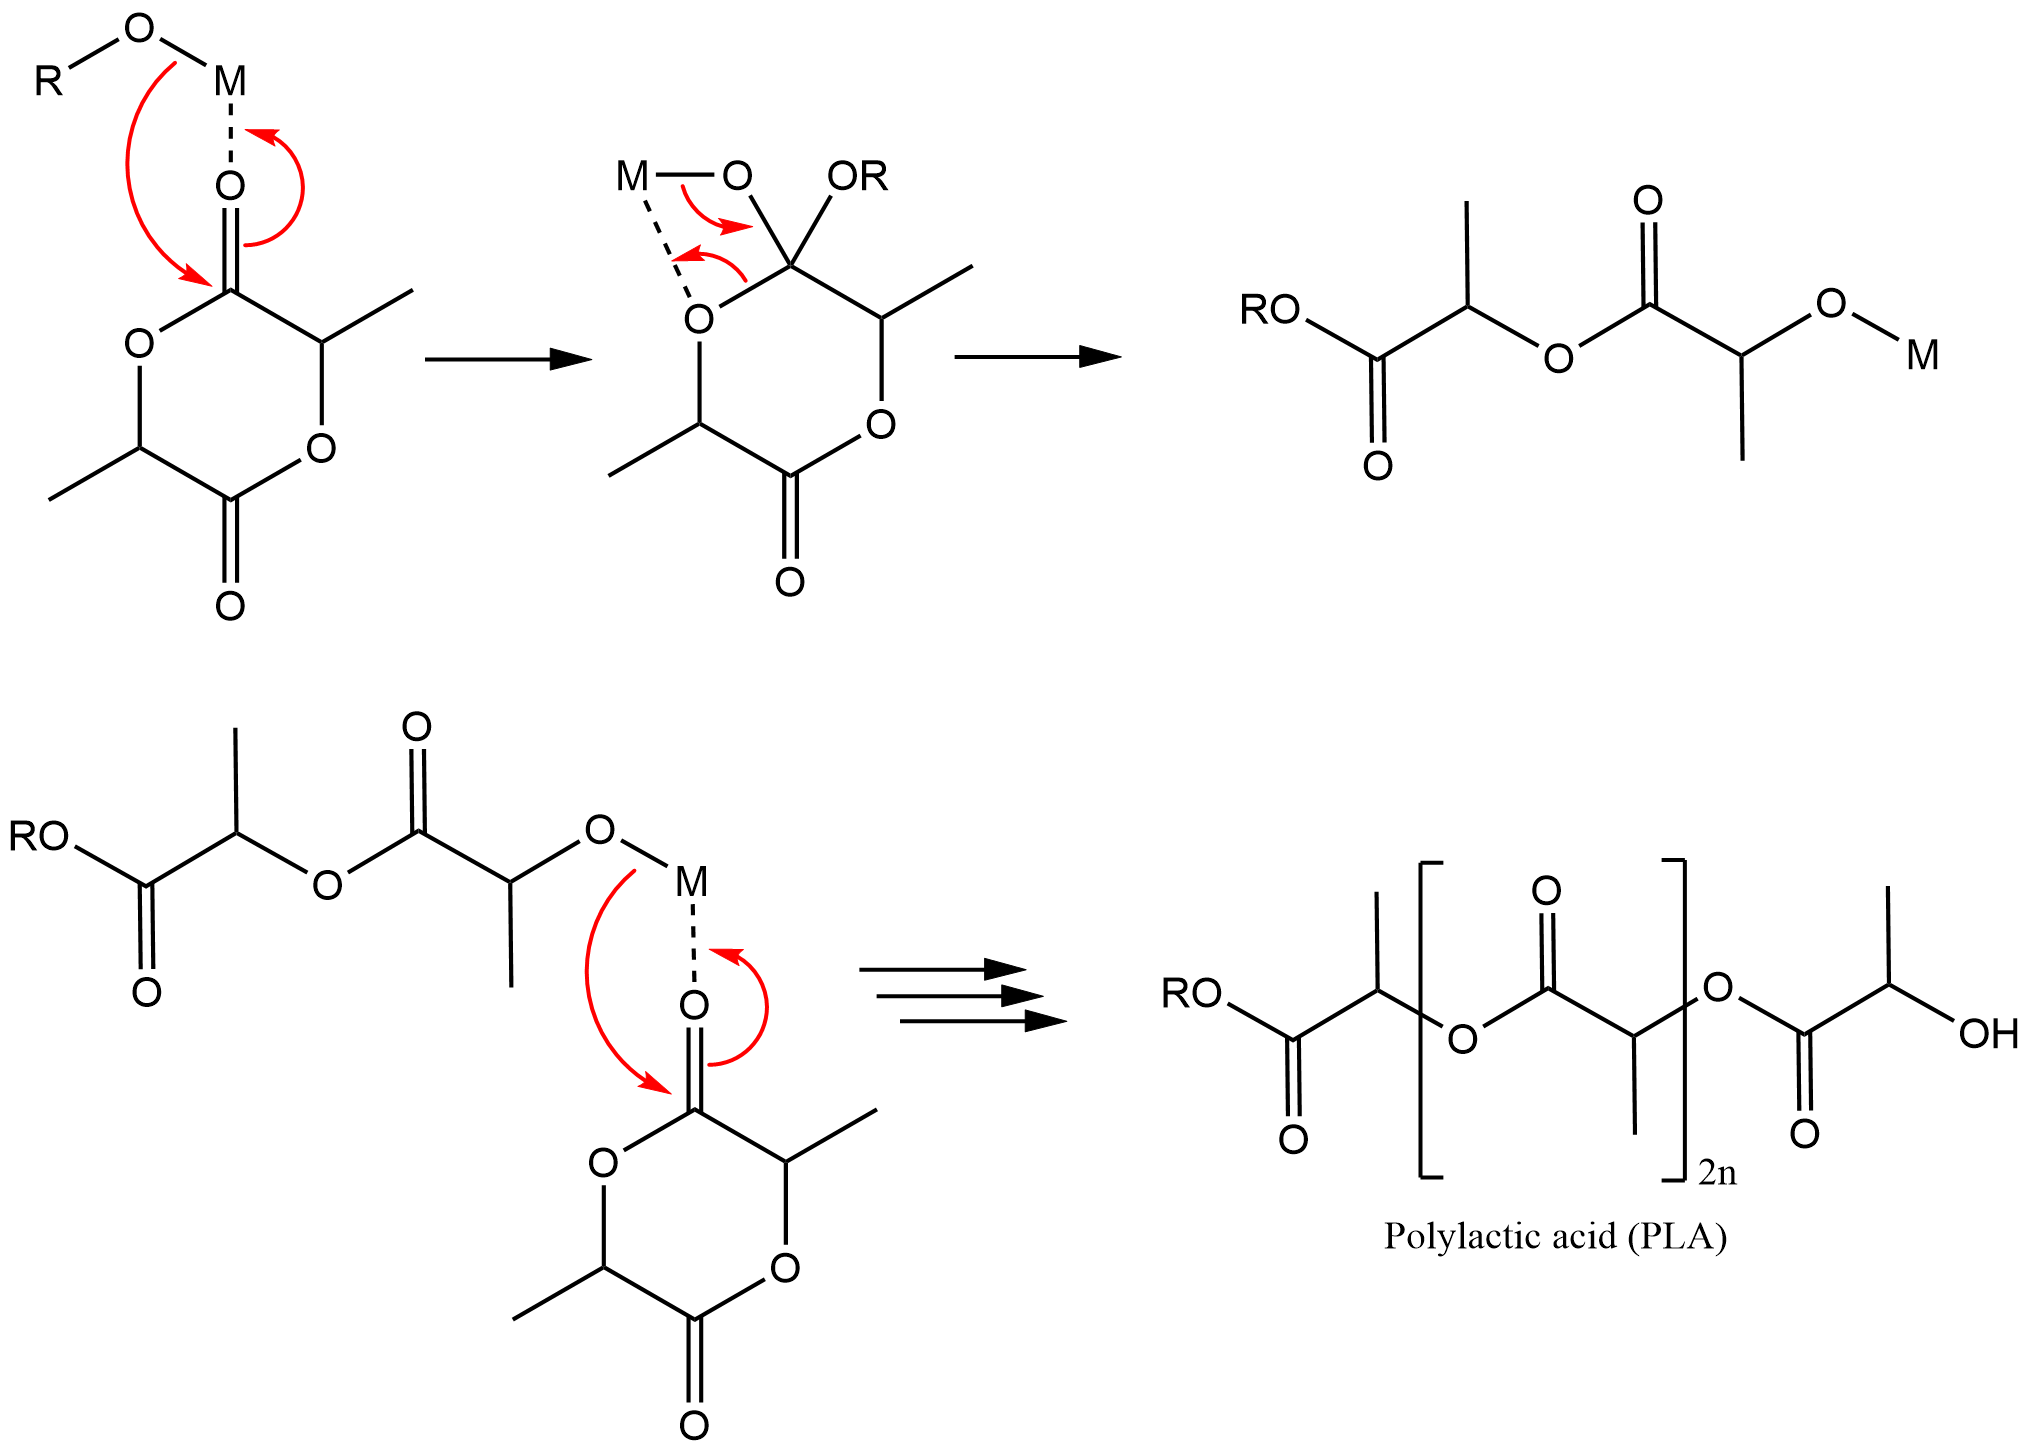
\includegraphics[width=0.8\textwidth]{PLA_ROP.png}
    \caption{ROP of lactide\citec{C0PY00204F}}
    \label{fig:PLA_ROP}
\end{figure}

\subsection{Polycondensation}

The most common mechanism of direct polycondensation of \gls{la} into \gls{pla} is depicted in figure \ref{fig:PLA_condensation}. It is an equilibrium reaction in which \gls{la} molecules bind together, releasing water molecules. Similar as to \gls{rop} does the choice of \gls{la} result in different types of \gls{pla}. 
The pure L- and D-\gls{la} results in \gls{plla} and \gls{pdla}, respectively, while the racemic mixture of the two results in \gls{pdlla}\citec{MASUTANI201411}. 

Polymers produced through direct polycondensation are usually of low molecular weight and low quality. Because of this newly developed polycondensation methods have been proposed such as \gls{ap} and \gls{ssp}. 

One of the benefits of \gls{rop} over polycondensation is the ability to produce polymers with a wider range of molecular weights by controlling the purity of lactide and the synthesis conditions, without the need for a chain coupling agent or an azeotropic system. 
Therefore, \gls{rop} is still the most common used mechanism in \gls{pla} leading producers\citec{chafran2019}.

\begin{figure}[ht]
    \centering
    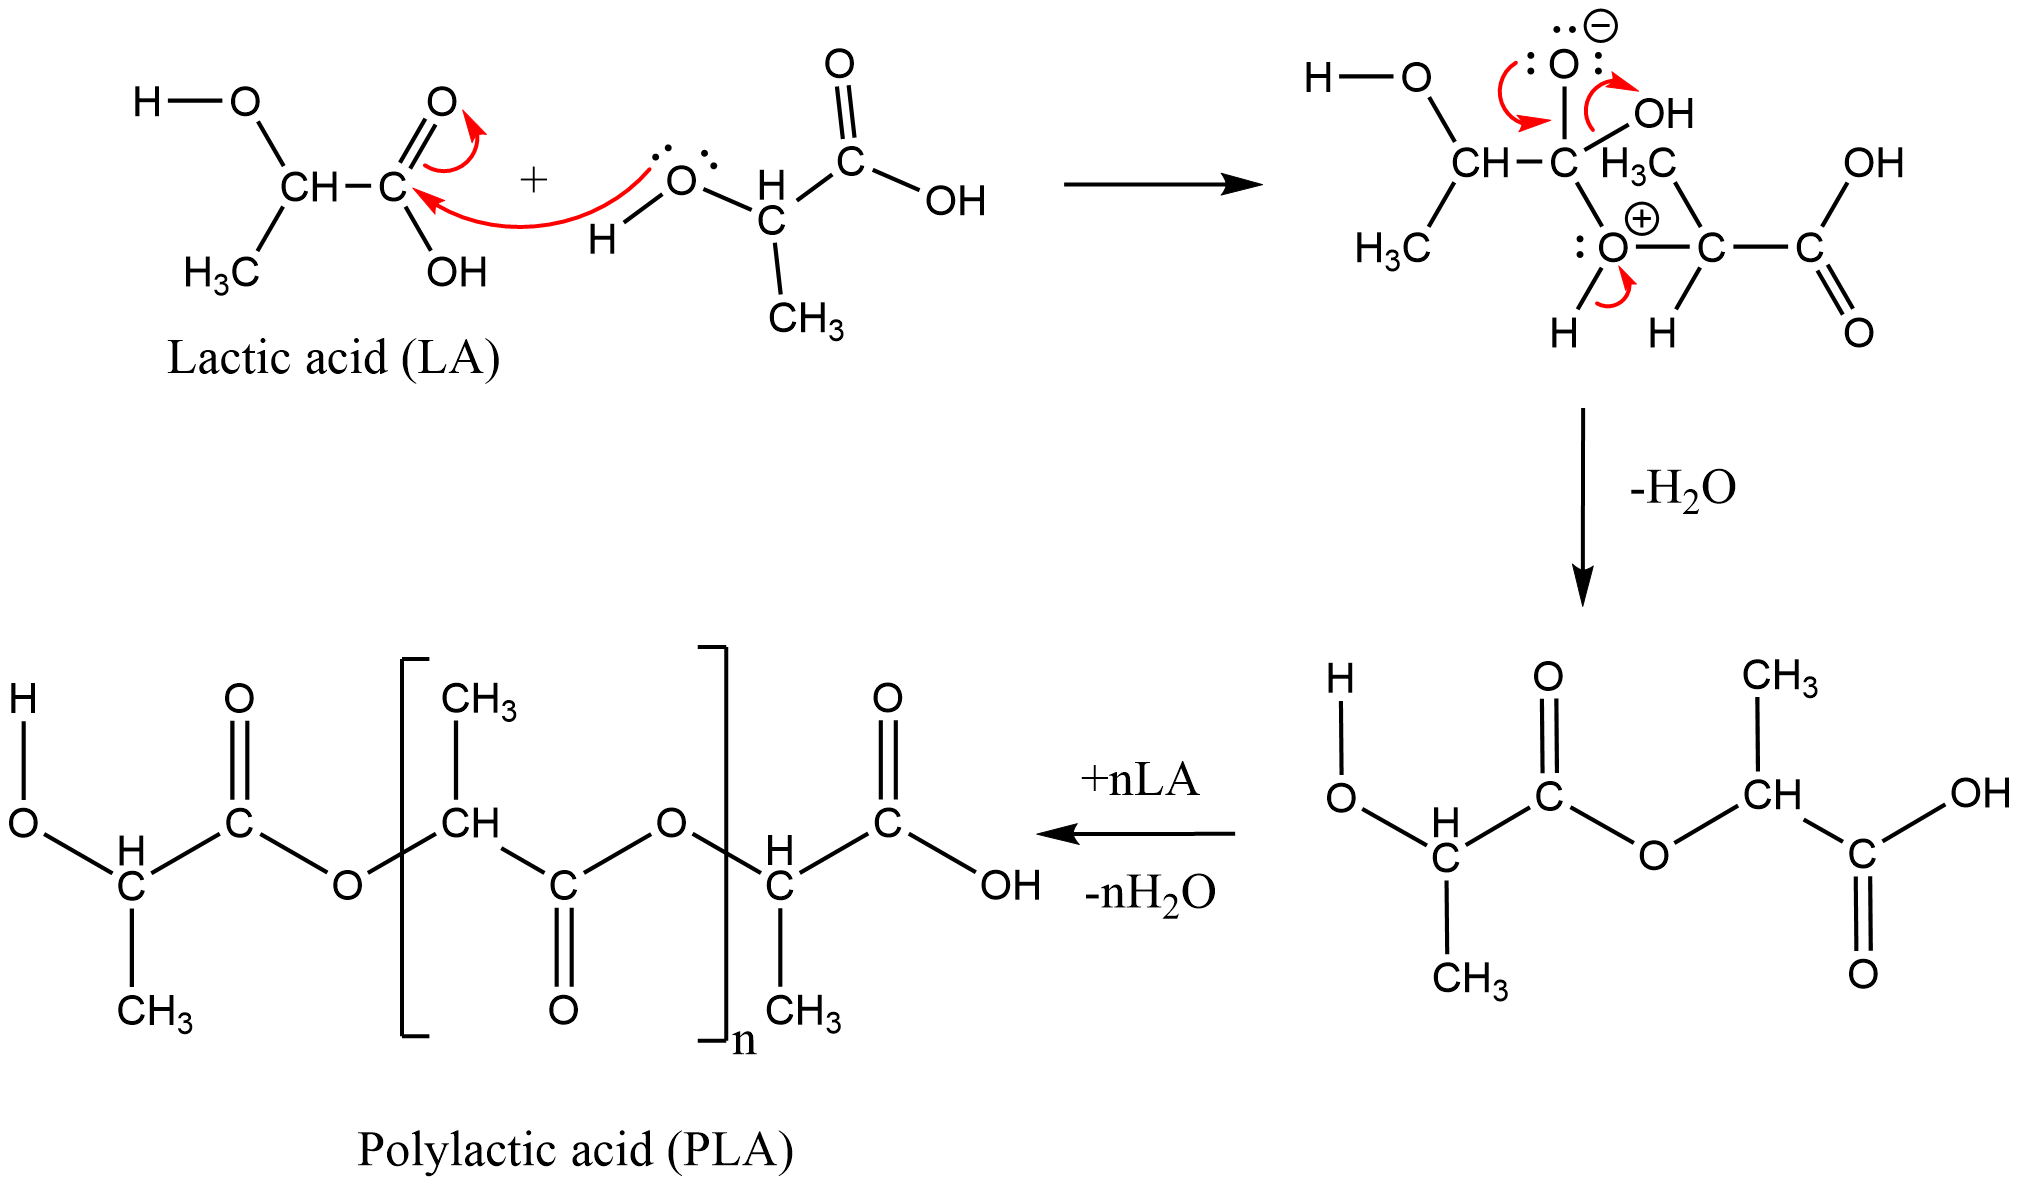
\includegraphics[width=0.8\textwidth]{PLA_condensation.png}
    \caption{Polycondensation polymerisation of PLA}
    \label{fig:PLA_condensation}
\end{figure}


\section{DSC and TGA techniques for 3D-printing of polymers}

A \gls{tga} measurement makes it possible to determine the temperature in which the polymer is stable, i.e. above some temperatures the polymer starts to degradate(fig. \ref{fig:TGA_DSC}). 
This information is important when 3D-printing techniques are used in which the polymer is subjected to higher temperatures. Furthermore, when a \gls{dsc} test would be performed it is important 
to know the bounds on the temperature. 

\gls{dsc} is usefull for 3D-printing since it gives information on how a sample physically and chemically changes upon endothermal or exothermal processes or changes in heat capacity. On figurre \ref{fig:TGA_DSC} the \gls{dsc} curve displays the differential heat flow in function of the temperature. 
The peaks indicate that the material undergoes a transition. This information is crucial for picking the right temperature in which the 3D-printing processes needs to take place\citec{JASON2022}.

\begin{figure}[ht]
    \centering
    \begin{subfigure}[b]{0.4\textwidth}
        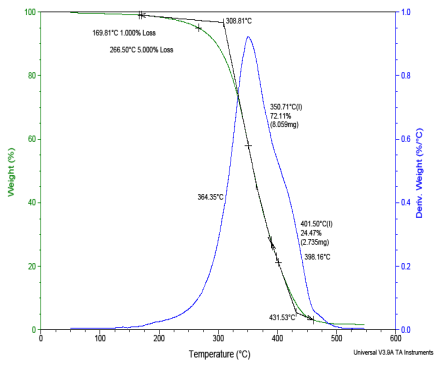
\includegraphics[width=\textwidth]{TGA.png}
    \end{subfigure}
    \begin{subfigure} [b]{0.5\textwidth}
        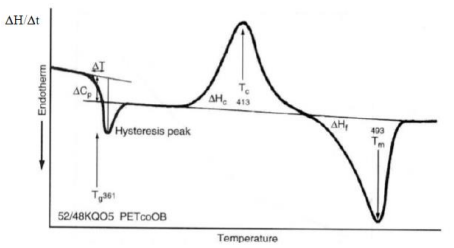
\includegraphics[width=\textwidth]{DSC.png}
    \end{subfigure}
    \caption{Typical TGA curve (left) and typical DSC curve (right)}
    \label{fig:TGA_DSC}
\end{figure}

\section{Group logo and dogbone design}

\subsection{Group logo}

\begin{figure}[H]
    \centering
    \begin{subfigure}[b]{0.4\textwidth}
        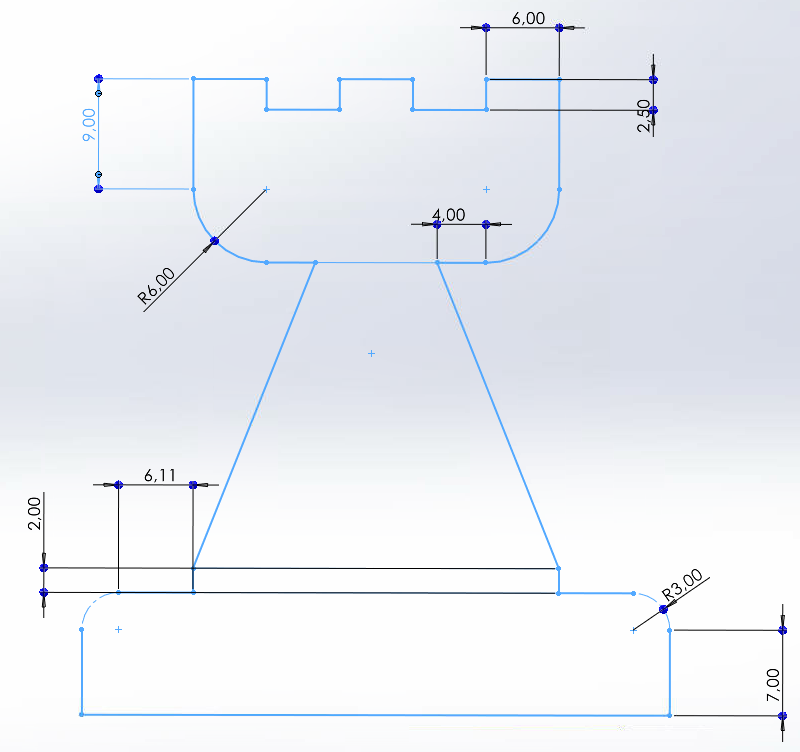
\includegraphics[width=\textwidth]{tower_sketch.png}
    \end{subfigure}
    \begin{subfigure}[b]{0.4\textwidth}
        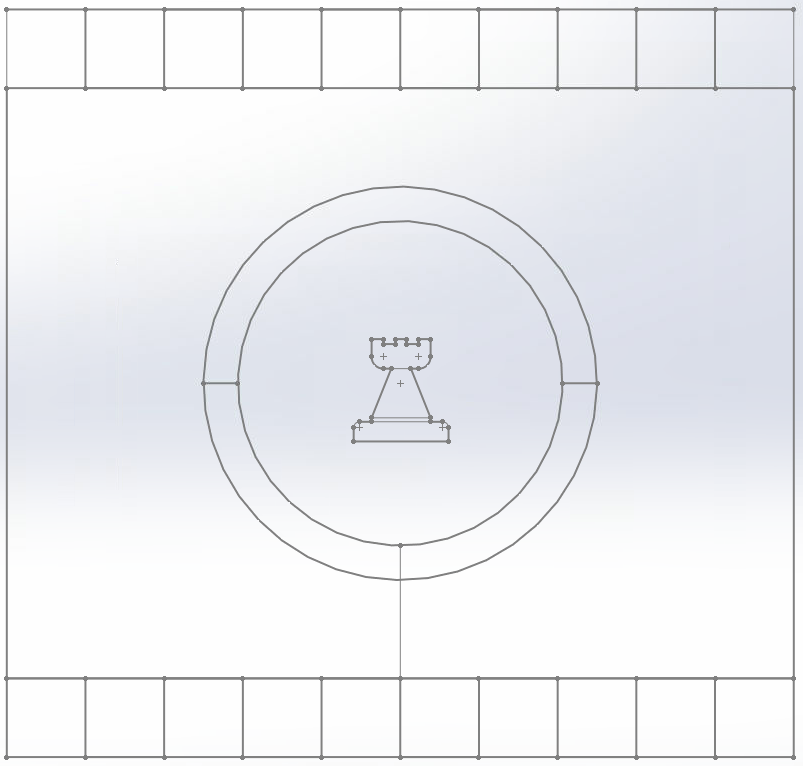
\includegraphics[width=\textwidth]{tower2D.png}
    \end{subfigure}
    \caption{tower dimensions (left) and tower logo (right)}
    \label{fig:tower}
\end{figure}

\begin{figure}[H]
    \centering
    \begin{subfigure}[b]{0.4\textwidth}
        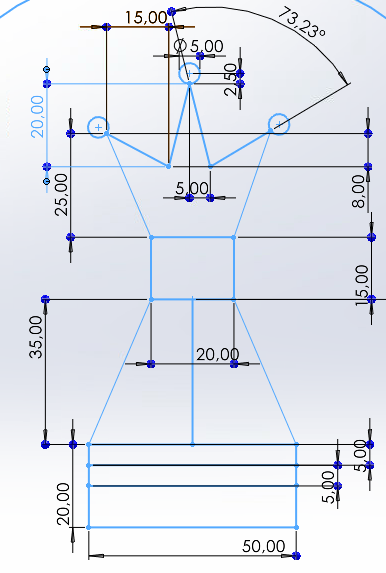
\includegraphics[width=\textwidth]{king_sketch.png}
    \end{subfigure}
    \begin{subfigure}[b]{0.45\textwidth}
        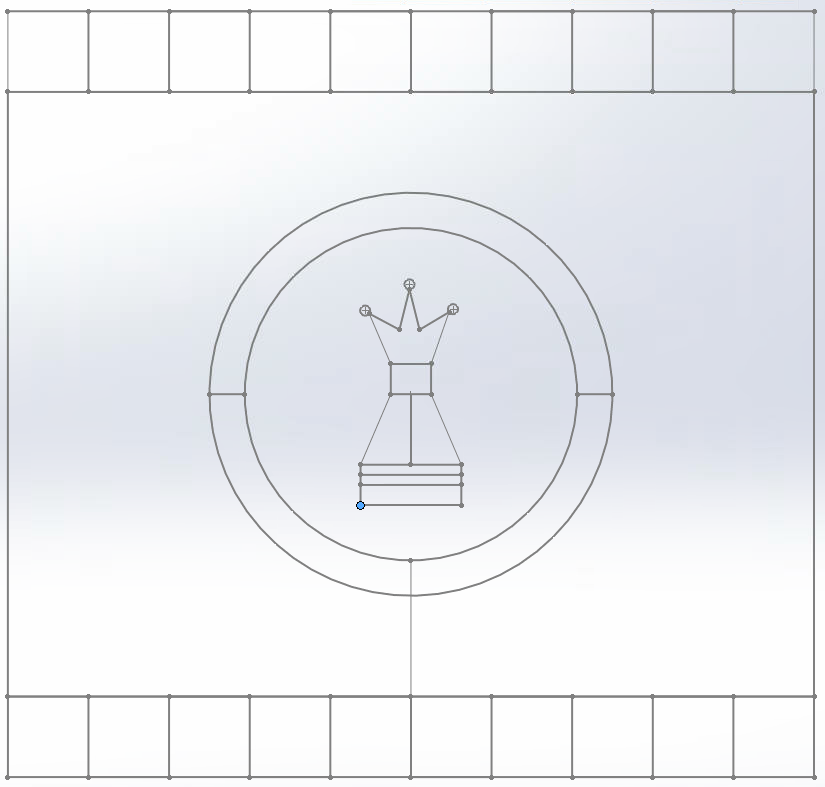
\includegraphics[width=\textwidth]{king2D.png}
    \end{subfigure}
    \caption{King dimensions (left) and king logo (right)}
    \label{fig:king}
\end{figure}

\begin{figure}[H]
    \centering
    \begin{subfigure}[b]{0.4\textwidth}
        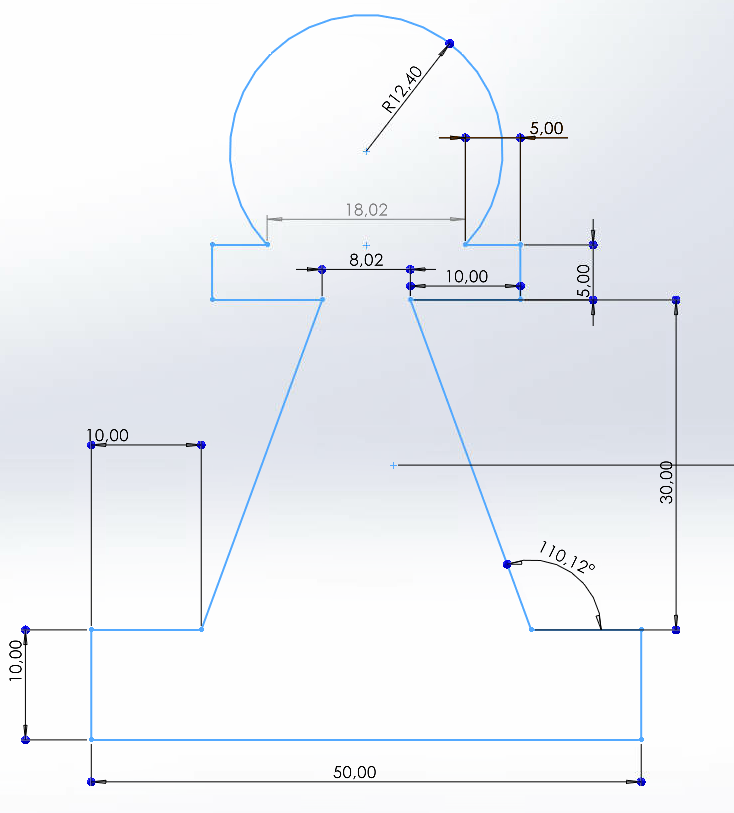
\includegraphics[width=\textwidth]{pion_sketch.png}
    \end{subfigure}
    \begin{subfigure}[b]{0.45\textwidth}
        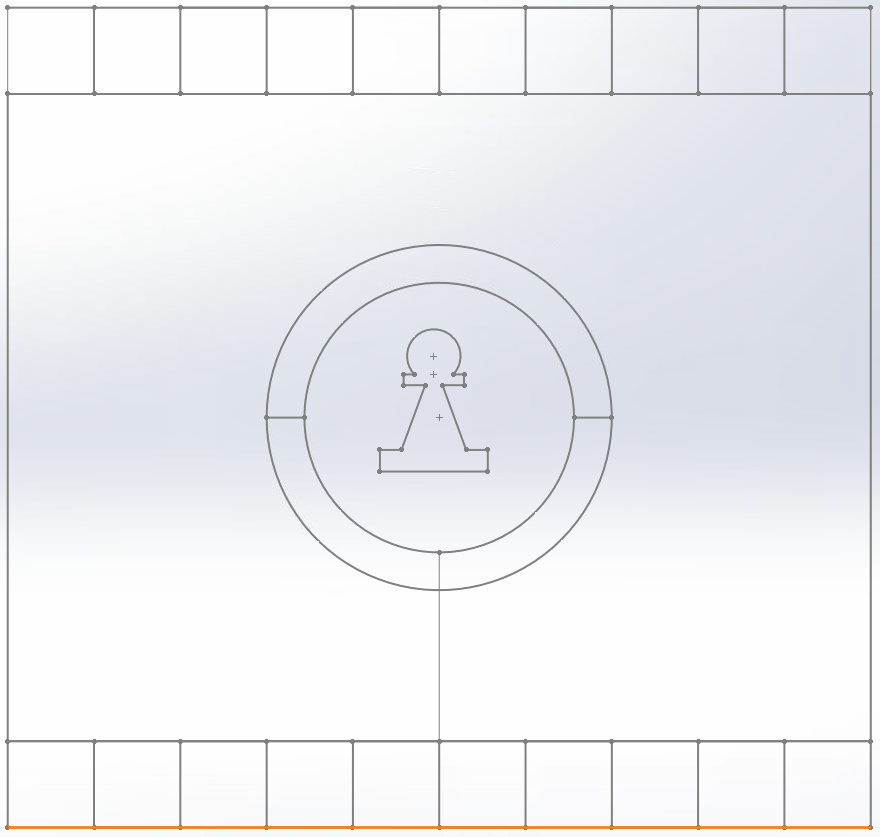
\includegraphics[width=\textwidth]{pion2D.png}
    \end{subfigure}
    \caption{Pawn dimensions (left) and pawn logo (right)}
    \label{fig:pawn}
\end{figure}

\subsection{Dogbone}

\begin{figure}[H]
    \centering
    \begin{subfigure}[b]{0.45\textwidth}
        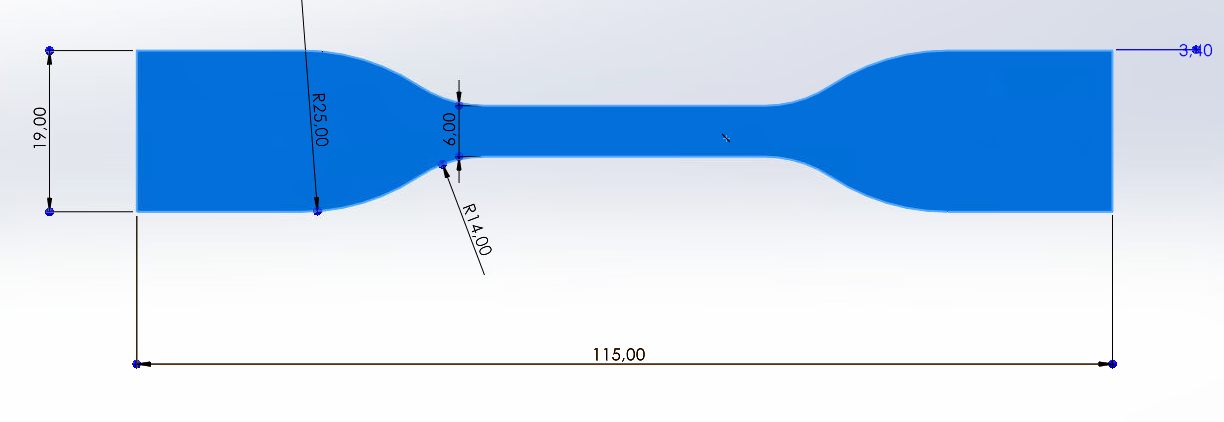
\includegraphics[width=\textwidth]{dogbone2D.png}
    \end{subfigure}
    \begin{subfigure}[b]{0.4\textwidth}
        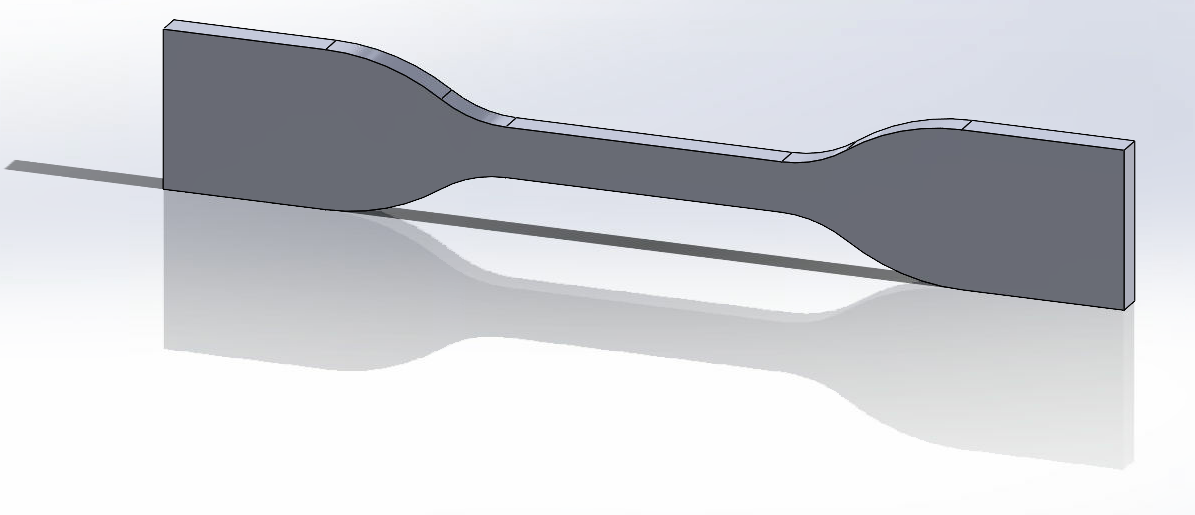
\includegraphics[width=\textwidth]{dogbone3D.png}
    \end{subfigure}
    \caption{Dogbone sketch (left) and dogbone 3D (right)}
    \label{fig:dogbone}
\end{figure}

\newpage
\bibliographystyle{plain}
\bibliography{mybib.bib}

\end{document}
